\chapter{Fourier Transform}
I am unsatisfied with the way Fourier transform is taught in most textbooks.
Both mathematical intuition and vigour are missing. I will explain
it in an intuitive way.

\section{What is Fourier Transform}

Think of sound or any signal (music, image, stock price) as a messy mixture of waves.

The Fourier transform is a tool that says:
Instead of looking at the signal over time (or space), let me break it into simple pure tones (sine waves).

\begin{figure}[ht]
\centering
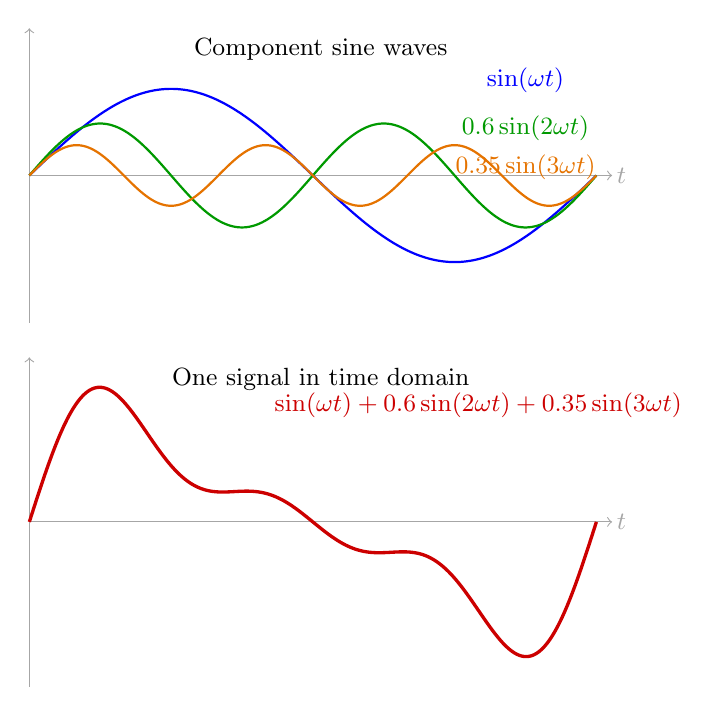
\begin{tikzpicture}[x=0.02cm,y=1.1cm]
  % Axes for component waves
  \draw[->,gray!70] (0,0) -- (370,0);
  \draw[->,gray!70] (0,-1.7) -- (0,1.7);
  \node[gray!70] at (376,0) {\small \(t\)};
  \node at (185,1.45) {\small Component sine waves};

  \draw[blue,thick,samples=220,domain=0:360] plot (\x,{sin(\x)});
  \draw[green!60!black,thick,samples=220,domain=0:360] plot (\x,{0.6*sin(2*\x)});
  \draw[orange!90!black,thick,samples=220,domain=0:360] plot (\x,{0.35*sin(3*\x)});

  \node[blue] at (315,1.1) {\small \(\sin(\omega t)\)};
  \node[green!60!black] at (315,0.55) {\small \(0.6\sin(2\omega t)\)};
  \node[orange!90!black] at (315,0.1) {\small \(0.35\sin(3\omega t)\)};

  % Axes for summed signal
  \begin{scope}[yshift=-4.4cm]
    \draw[->,gray!70] (0,0) -- (370,0);
    \draw[->,gray!70] (0,-1.9) -- (0,1.9);
    \node[gray!70] at (376,0) {\small \(t\)};
    \node at (185,1.65) {\small One signal in time domain};

    \draw[red!80!black,very thick,samples=300,domain=0:360]
      plot (\x,{sin(\x)+0.6*sin(2*\x)+0.35*sin(3*\x)});

    \node[red!80!black] at (285,1.35)
      {\small \(\sin(\omega t)+0.6\sin(2\omega t)+0.35\sin(3\omega t)\)};
  \end{scope}
\end{tikzpicture}
\caption{A single signal can be represented as the sum of multiple sine waves with different frequencies and amplitudes.}
\end{figure}

It is like
\begin{itemize}
\item Taking a chord on a piano and asking: which notes are being played, and how loud is each note?
The chord sounds like one object to your ear, but it is actually a sum of several pure tones.
\item Taking white light and passing it through a prism: one beam becomes many colors.
The original light is still the same physical signal, but now you can see its components separately.
\item Looking at ocean waves from far away: the surface looks irregular, but you can still describe it as a blend of slow, medium, and fast wave patterns.
\end{itemize}

So:
\begin{itemize}
\item Input: a signal in time (or space), such as sound pressure, pixel brightness, or voltage.
\item Output: a frequency description that tells:
  \begin{itemize}
  \item which frequencies are present,
  \item how strong each frequency is (amplitude or energy),
  \item and, in the complex form, how each frequency is shifted (phase).
  \end{itemize}
\item Interpretation: a peak at a frequency means that frequency plays an important role in building the original signal.
\end{itemize}

Why is this useful?

Because many problems become easier when you look at frequencies instead of time.

Examples:
\begin{itemize}
\item \textbf{Music and audio:} detect pitch, remove noise, and compress files (for example, MP3 keeps important frequency content and discards less important parts).
\item \textbf{Images:} blur and sharpen filters become simple frequency operations; JPEG-style compression works by keeping the strongest visual frequency components.
\item \textbf{Medical imaging:} MRI data is collected in a frequency-like domain and then transformed back to produce a spatial image.
\item \textbf{Physics and engineering:} vibrations of strings, bridges, and machines are understood through dominant frequencies and resonance.
\end{itemize}

\section{Linear Space}
A vector is the plane can be represented as weighted sum of two
orthogonal base vectors.
\[
\mathbf{v} = x\mathbf{v_1} + y\mathbf{v_2}
\]
Orthogonal means the two vectors are perpendicular to each other. In mathematic
terms, the inner product of the two vectors is zero.

\[
<\mathbf{v_1} ,\mathbf{v_2}> = 0
\]

For example, we can place \(v_1\) along the x-axis and \(v_2\) along the y-axis. Obviously
they are perpendicular to each other.

The weights are the projections of the vector onto the orthogonal vectors,
which are the dot products of the vector with the orthogonal vectors.
\[
\mathbf{v} = \mathbf{(x,y)} = x\mathbf{(1,0)} + y\mathbf{(0,1)}
\]
\[
x = \mathbf{v} \cdot \mathbf{(1,0)}
\]
\[
y = \mathbf{v} \cdot \mathbf{(0,1)}
\]

The inner product is a mathematical operation that takes two vectors and returns a scalar.
It generalizes the dot product and is defined in a vector space, satisfying properties such as linearity, symmetry, and positive definiteness. The inner product allows for the formal definition of geometric concepts like lengths, angles, and orthogonality of vectors.
The inner product of \(v_1\) and \(v_2\) is written as \(<v_1, v_2>\).

Generally, an n-dimensional vector can be represented as a weighted sum of n orthogonal bases:
\[
\mathbf{v} = \sum_{i=1}^n c_i \mathbf{e_i}
\]
\[
<\mathbf{e_i}, \mathbf{e_j}> = 0 \text{ if } i \neq j
\]
\[
c_i = \frac{<\mathbf{v}, \mathbf{e_i}>}{<\mathbf{e_i}, \mathbf{e_i}>}
\]

\section{Linear Space and Fourier Transform}
We will show that a signal in time domain can be represented as a weighted sum of sine waves
as a vector is represented as a weighted sum of orthogonal bases.
We use complex value so sine wave becomes complex exponential function.
In reality, the frequency is continuous. So we use integral instead of sum:

\[
f(t) = \int_{-\infty}^{\infty} F(f) e^{i2\pi f t} df
\]

The bases are
\[
e^{i2\pi f t}
\]

For complex-valued signals, the natural inner product uses complex conjugation
(so lengths are real and nonnegative):
\[
<f, g> = \int_{-\infty}^{\infty} f(t)\,\overline{g(t)}\, dt
\]

The inner product of two different frequency ``basis'' exponentials is zero
when \(f\neq g\):
\[
<e^{i2\pi f t}, e^{i2\pi g t}> = 0
\]

Why? Expand using the definition above:
\[
\begin{aligned}
& <e^{i2\pi f t}, e^{i2\pi g t}> \\
&= \int_{-\infty}^{\infty} e^{i2\pi f t}\, e^{-i2\pi g t}\, dt \\
&= \int_{-\infty}^{\infty} e^{i2\pi (f-g) t}\, dt.
\end{aligned}
\]
When \(f\neq g\), the integrand oscillates evenly around zero: over each cycle,
the positive and negative parts cancel, so there is no net ``overlap'' between
the two pure tones. In the continuous-frequency theory, this orthogonality is
made precise by the delta identity: the integral above behaves like
\(\delta(f-g)\), which is zero when \(f\neq g\) (and is singular at \(f=g\),
where the two exponentials match). Intuitively: different frequencies are
orthogonal directions in an infinite-dimensional space, just as different
coordinate axes are perpendicular in the plane.

As in linear space, the weighted sum is the inner product of the signal with the sine waves.
We call it Fourier transform:
\[
F(f) = \int_{-\infty}^{\infty} f(t) e^{-i2\pi f t} dt
\]

The original signal is the sum of weighted sine waves. We call it inverse Fourier transform:
\[
f(t) = \int_{-\infty}^{\infty} F(f) e^{i2\pi f t} df
\]
